
设计C++程序时,性能通常是一个关键因素。虽然在单个应用范围内使用该语言可能会有很长的路要走,但适当的高级设计对于实现最佳延迟和吞吐量很重要。先来讨论几个关键的模式。

\subsubsubsection{4.5.1\hspace{0.2cm}CQRS和事件源}

有许多方法可以扩展计算,但扩展数据访问可能很棘手。然而,当用户基础增长时,这通常是必要的。\textbf{命令查询责任分离(CQRS)}模式可以在这里可以提供帮助。

\hspace*{\fill} \\ %插入空行
\noindent
\textbf{命令-查询式责任分离}

传统的CRUD系统中,读和写都使用相同的数据模型和数据流,并以相同的方式执行。名义上的隔离意味着可以以两种不同的方式处理查询(读取)和命令(写入)。

许多应用程序的读和写的比例偏差很大——通常的应用程序中,从数据库中读取的数据比更新数据库的数据要多得多。这意味着需要尽可能快地读取数据,从而有更好的性能:读和写现在可以分别进行优化和扩展。更重要的是,如果许多写操作相互竞争,或者需要维护所有写操作的轨迹,或者一组API用户应该具有只读访问权限,那么引入CQRS可能会有所帮助。

拥有独立的读和写模型可以让不同的团队在分开工作。从事读取方面工作的开发人员不需要对领域有深入的了解,这是正确执行更新所必需的。当他们发出请求时,只需要一个简单的调用就可以读取层得到一个\textbf{数据传输对象(DTO)},而非通过域模型。

如果不知道DTO是什么,可以考虑从数据库返回项目数据。如果调用者要求一个项目列表,可以提供一个只包含项目名称和缩略图的\textit{ItemOverview}对象。另一方面,如果想要特定商店的商品,也可以提供一个包含名称、更多图片、描述和价格的\textit{StoreItem}对象。\textit{ItemOverview}和\textit{StoreItem}都是DTO,从数据库中相同的\textit{Item}对象中抓取数据。

读取层可以位于用于写的数据存储的顶部,也可以是通过事件更新的不同的数据存储,如图4.2所示。

使用图4.2中所示的方法,可以创建多个不同的命令,每个命令都有自己的处理程序。命令是异步的,不会向调用者返回。每个处理程序都使用域对象,并会等待更改完成。之后,将发布事件,事件处理程序可用于更新读取操作使用的存储。继续上一个示例,项目数据查询将从由诸如\textit{ItemAdded}或\textit{ItemPriceChanged}等事件更新的数据库中获取信息,这些事件可以由\textit{AddItem}或\textit{ModifyItem}等命令触发。

使用CQRS可以为读写操作使用不同的数据模型。例如,可以创建存储过程和物化视图来加速读取。对于读存储和域存储,使用不同类型的存储(SQL和NoSQL)也有好处:持久化数据的一种方法是使用Apache Cassandra集群,而使用Elasticsearch是快速搜索存储数据的一种不错的方法。

除了前面的优点,CQRS也有它的缺点。由于其引入的复杂性,通常不适合小型或要求较少的架构。还有,在域存储之后更新读存储,数据有一致性,但不是强一致性。

\begin{center}
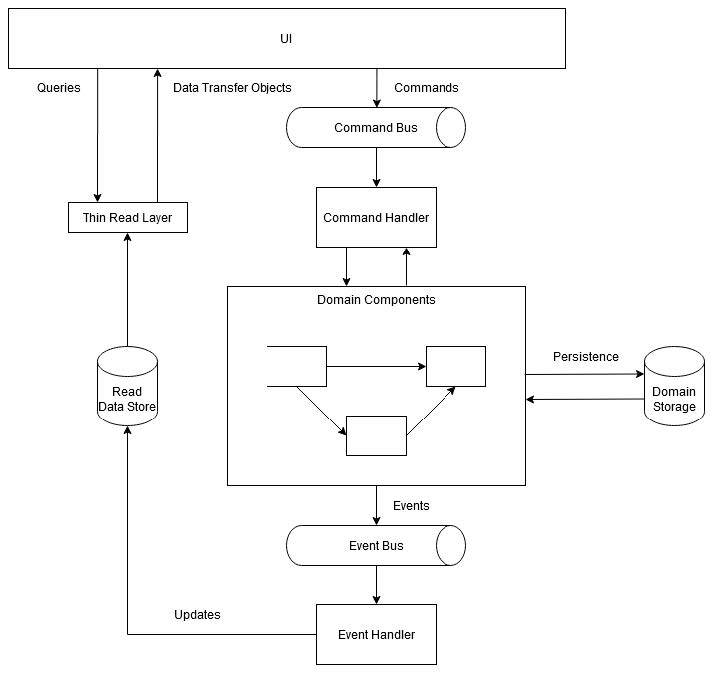
\includegraphics[width=0.9\textwidth]{content/2/chapter4/images/2.jpg}\\
图4.2 -带有事件源的CQRS
\end{center}

\hspace*{\fill} \\ %插入空行
\noindent
\textbf{命令-查询式分离}

CQRS实际上基于很久以前在Eiffel编程语言中引入的一个更简单的思想(与引入契约的思想相同)。\textbf{命令查询分离(CQS)}是一个原则,设计分离API调用。命令和查询-就像在CQRS,但不考虑规模,在目标编程和命令式编程中都发挥得很好。

如果函数名以\textit{has},\textit{is},\textit{can}或类似的单词开头,那应该只是一个查询,而不会对底层状态进行修改或有其他副作用。这带来了两个好处:

\begin{itemize}
\item 
\textbf{代码更易读}: 这样的函数在语义上只是\textit{read},而不是\textit{write}。这使得在调试时查找状态变化更加容易。

\item 
\textbf{减少海森堡bug}: 如果需要调试在发布版本中出现的错误,但在调试版本中却没有(或者相反),这就已经处理了一个海森堡bug。这很少是令人愉快的事情。许多这样的错误可能是由修改状态的断言引起的。遵循CQS可以消除这样的bug。
\end{itemize}

与断言类似,如果想要使用契约(前置条件和后置条件),那么只在其中使用查询非常重要。否则,禁用一些契约检查也可能导致海森堡bug,更不用说这将是多么的违反直觉。

现在,来了解一下事件源。

\hspace*{\fill} \\ %插入空行
\noindent
\textbf{事件源}

如在第2章所述,事件源可以只存储发生在应用程序状态上的更改,而不是总是存储应用程序的整个状态(可能在更新期间处理冲突)。使用事件源可以通过消除并发更新和允许所有感兴趣的方对其状态执行,逐步更改来提高应用程序的性能。保存所做操作的历史记录(例如,市场交易)可以更容易地进行调试(通过稍后重播)和审核。这也带来了更多的灵活性和扩展性。引入事件源时,一些域模型可以变得更简单。

事件源的成本是最终保持一致。另一个问题是降低应用程序的启动速度——除非对状态进行定期快照,或者可以使用CQRS中的只读存储,上一节已经讨论过。

好了,关于CQRS和相关模式已经了解了。现在转向另一个有关性能的话题:缓存。

\subsubsubsection{4.5.2\hspace{0.2cm}缓冲}

正确地使用缓存可以产生更好的性能、更低的延迟、减少服务器负载(在云中运行的成本),并有助于解决可扩展性问题(所需的服务器更少)。

\begin{tcolorbox}[colback=blue!5!white,colframe=blue!75!black, title=Note]
\hspace*{0.75cm}如果在寻找CPU缓存的技巧,可以在\textit{第11章}了解到相关信息。
\end{tcolorbox}

缓存是一个大主题,在这里只讨论几个方面。

缓存的工作原理是,将最常读取的数据存储在访问时间较短的非持久存储中。有许多不同类型的缓存:

\begin{itemize}
\item 
\textbf{客户端缓存}: 用于专门为给定客户存储数据,通常放置在客户机或浏览器上。

\item 
\textbf{Web服务器缓存}: 为了加速网页的阅读,可以通过Varnish这样的HTTP加速器来缓存Web服务器的响应。

\item
\textbf{数据库缓存}: 许多数据库引擎都有内置的、可调优的缓存。

\item
\textbf{应用程序缓存}: 为了加速应用程序,可以从缓存读取数据,而不是从数据库读取数据。

\item
\textbf{CDN也可以视为缓存}: 从靠近用户的位置提供内容,以减少延迟。
\end{itemize}

可以在集群中复制或部署某些类型的缓存,以提供大规模性能。另一种选择是进行分片:类似于对数据库进行分片,可以为数据的不同部分使用缓存的不同实例。

现在了解一下更新缓存中的数据的不同方法。毕竟,没有人喜欢旧数据。

\hspace*{\fill} \\ %插入空行
\noindent
\textbf{更新缓存}

有几种方法可以保持缓存数据的新鲜度。无论决定更新缓存项的人还是其他公司,对其进行了解都是很有意义的。本节中,将讨论它们的优缺点。

\hspace*{\fill} \\ %插入空行
\noindent
\textit{直写模式}

如果需要强一致性,同步更新数据库和缓存是有效的方法。这种方法可以防止数据丢失:如果数据对用户可见,就已经写入数据库。直写缓存的缺点是,执行更新的延迟比其他方法更大。

\hspace*{\fill} \\ %插入空行
\noindent
\textit{滞后写}

另一种方法,也称为回写,是只向用户提供对缓存的访问。当用户执行更新时,缓存将对传入的更新进行排队,然后将异步执行该更新,从而更新数据库。缺点是,如果出现错误,就永远不能写入数据。它也不像其他方法那样容易实现。但是,好处是用户看到的延迟最低。

\hspace*{\fill} \\ %插入空行
\noindent
\textit{缓存延迟}

最后一种方法,也称为\textbf{延迟加载},是关于按需填充缓存的。这种情况下,数据访问如下所示:

\begin{enumerate}
\item 
调用缓存来检查值是否已经存在。如果是,就返回。

\item 
提供值的主数据存储或服务。

\item
将值存储在缓存中,并返回给用户。
\end{enumerate}

这种类型的缓存通常使用Memcached或Redis,可以非常快速和高效—缓存只包含请求的数据。

但是,如果经常请求不在缓存中的数据,则前三个调用会显著增加延迟。为了减轻缓存重启的影响,可以用持久存储中选定的数据初始化(初始化)缓存。

缓存中的项也可能过时,因此最好为每个条目设置生存时间。如果要更新数据,可以采用直写的方式,即从缓存中删除记录并在数据库中更新它。当只使用基于时间的更新策略(例如,在DNS缓存中)使用多级缓存时要小心。这可能导致长时间使用旧数据。

已经讨论了缓存的类型和更新它们的策略,所以关于缓存的内容就到此为止。接下来,讨论扩展架构的另一个方面。






